\documentclass{book}
\usepackage[english]{babel}
\usepackage[utf8]{inputenc}

\usepackage{graphicx,tikz,wrapfig,hyperref,fancybox}
\renewcommand{\(}{\begin{columns}}
\renewcommand{\)}{\end{columns}}
\newcommand{\<}[1]{\begin{column}{#1}}
\renewcommand{\>}{\end{column}}
\newcommand{\lien}[2]{\mathcal{L}_{#1}^{#2}}
\newcommand{\lie}[1]{\mathcal{L}_{#1}}
\newcommand{\colv}[2]{\begin{pmatrix}#1\\#2\end{pmatrix}}

\begin{document}

\chapter{Introduction}
\section{Overview}
% Piecewise smooth dynamical systems
Theory of dynamical systems enables us to gain valuable insights into many problems.  By using the powerful 
tools it provides, in many cases we can explain how a system will behave 
when the actual equations governing its evolution are too difficult to solve 
analytically.  This approach has been proved time and again to be extremely 
useful in a diverse range of areas: fluid flows, electrical circuits, 
ecological systems etc.  

However, conventional treatments of the subject generally places the demand 
that the systems be describable in terms of \emph{smooth} functions of the 
dynamical variables. There are valid reasons for doing so.  For a system's 
stability analysis, the Jacobian plays a role of paramount importance.  But 
its existence cannot be guaranteed everywhere in the phase space for non 
smooth systems.  

Unfortunately, many systems we need to deal with regularly are non smooth: 
electrical circuits involving switches, systems exhibiting sliding or 
chattering motion, impacting systems etc.  One subclass of these systems is called  \emph{piecewise smooth} systems. The equation governing the evolution

\begin{figure}
\caption{Trajectory of a bouncing ball : a piecewise smooth system}
\begin{center}
\includegraphics[width=0.4\columnwidth]{bounce}
\end{center}
\end{figure}
 
of these system changes the moment  the system 
co-ordinates cross what is known as a ``switching manifold'', which is a 
surface with 
dimension lower than that of the phase space.  Between any two of those 
switches, the system evolves smoothly.  

% Examples
% Behaviours specific to it: border collision
% Order of discontinuity: trace and Jacobian
% ZDM approach
% Chaos narrow band vanishing for integer n : hole: no chaos unexplained
% Impact map.  Budd et al: hole: no damping
% Numerical computation of fixed pt and jacobian 
% Transient lifetimes : unexplored


\chapter{Our system}
% description
% solution x_h and x_p
% approx poincare map
% impact map
% plot of numerical poincare map
% long transients
% hypothesis
% jacobians crossing 1
% FP losing stability?

\end{document}
